\documentclass[tikz]{standalone}

\usepackage[latin1]{inputenc}
\usepackage{tikz}
\colorlet{myblue}{cyan!40!white}
\usetikzlibrary{quotes,angles,calc,decorations.markings}
% GNUPL
% Draw line annotation
% Input:
%   #1 Line offset (optional)
%   #2 Line angle
%   #3 Line length
%   #5 Line label
% Example:
%   \lineann[1]{30}{2}{$L_1$}
\newcommand{\lineann}[4][0.5]{%
    \begin{scope}[rotate=#2, blue,inner sep=2pt]
        \draw[densely dashed, blue!40] (0,0) -- +(0,#1)
            node [coordinate, near end] (a) {};
        \draw[densely dashed, blue!40] (#3,0) -- +(0,#1)
            node [coordinate, near end] (b) {};
        \draw[|<->|] (a) -- node[] {\contour{white}{#4}} (b);
    \end{scope}
}
\newcommand{\lineannOnly}[4][0.5]{%
    \begin{scope}[rotate=#2, blue,inner sep=2pt]
        \draw[densely dashed, blue!40] (0,0) -- +(0,#1)
            node [coordinate, near end] (a) {};
        \draw[densely dashed, blue!40] (#3,0) -- +(0,#1)
            node [coordinate, near end] (b) {};
        % \draw[|<->|] (a) -- node[] {\contour{white}{#4}} (b);
    \end{scope}
}
\usepackage[outline]{contour}
\contourlength{2.1pt}
\begin{document}
\pagestyle{empty}


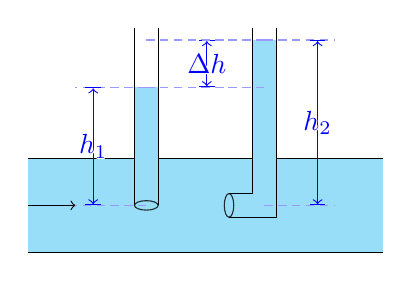
\begin{tikzpicture}[
    scale=1.5, 
    arrowline/.style={black!60},
    kos/.style={black},
    tangent/.style={
        decoration={
            markings,% switch on markings
            mark=
                at position #1
                with
                {
                    \coordinate (tangent point-\pgfkeysvalueof{/pgf/decoration/mark info/sequence number}) at (0pt,0pt);
                    \coordinate (tangent unit vector-\pgfkeysvalueof{/pgf/decoration/mark info/sequence number}) at (1,0pt);
                    \coordinate (tangent orthogonal unit vector-\pgfkeysvalueof{/pgf/decoration/mark info/sequence number}) at (0pt,1);
                }
        },
        postaction=decorate
    },
    use tangent/.style={
        shift=(tangent point-#1),
        x=(tangent unit vector-#1),
        y=(tangent orthogonal unit vector-#1)
    },
    use tangent/.default=1
    ]

% \draw[rotate=-30] (0,0) arc [ start angle=0,   
%                               end angle=360,
%                               x radius=0.5, 
%                               y radius=1]
%         coordinate [pos=0.06,sloped] (1a) {}  
%         coordinate [pos=-0.06,sloped] (1b) {} 
%         coordinate [pos=.235] (2) {}  
%         coordinate [pos=.5] (3) {} 
%         coordinate [pos=.76] (4) {};

% \draw (3) node[left=0.5em] {$S_1$};

% \draw[rotate around={-10:(2,-1)}, xshift=3cm, scale=0.4, yshift=-2cm] (0,0) arc [ start angle=0,   
%                               end angle=360,
%                               x radius=0.5, 
%                               y radius=1]
%         coordinate [pos=0] (1') {} 
%         coordinate [pos=.25] (2') {} 
%         coordinate [pos=-0.56,sloped] (3'a) {} 
%         coordinate [pos=0.56,sloped] (3'b) {} 
%         coordinate [pos=.75] (4') {} node[right] {$S_2$};

% % \draw (1) to [out=-30, in=180-10] (1');
% \draw (2) to [out=-40, in=180-10] node[sloped,pos=0.5]{\tikz{\draw[->](0,0) -- ++(0.1,0)}} (2');
% \draw (4) to [out=-20, in=180] node[sloped,pos=0.5]{\tikz{\draw[->](0,0) -- ++(0.1,0)}} (4');

% \draw (1a) to [out=-35, in=180-10] node[sloped,pos=0.5]{\tikz{\draw[->](0,0) -- ++(0.1,0)}} (3'a);
% \draw (1b) to [out=-25, in=180-5] node[sloped,pos=0.5]{\tikz{\draw[->](0,0) -- ++(0.1,0)}} (3'b);

% \draw[densely dashed] (3) to [out=-35, in=180-5]  (1');

% \begin{scope}
%     \clip[rotate=-30] (0,0) arc [ start angle=0,   
%                               end angle=360,
%                               x radius=0.5, 
%                               y radius=1];
% \draw[] (3) to [out=-35, in=180-5]  (1');
% \end{scope}
% \begin{scope}
%     \clip[rotate around={-10:(2,-1)}, xshift=3cm, scale=0.4, yshift=-2cm] (0,0) arc [ start angle=0,   
%                               end angle=360,
%                               x radius=0.5, 
%                               y radius=1];
% \draw[] (3) to [out=-35, in=180-5]  (1');
% \end{scope}

\draw[draw=none,fill=myblue] (0,0) rectangle (3,0.8);
\draw (0,0) -- ++(3,0);
\draw (0,0.8) -- ++(1-0.1,0) ++ (0.2,0) -- ++(1-0.2,0) ++ (0.2,0) -- ++ (0.9,0);

\draw[fill=myblue,draw=none] (1-0.1,0.4) rectangle ++(0.2,1);
\draw[black] (1-0.1,0.4) -- ++(0,1.5);
\draw[black] (1+0.1,0.4) -- ++(0,1.5);

\draw[fill=myblue,draw=none] (2-0.1,0.4) rectangle ++(0.2,1.4);
\draw[black] (2-0.3,0.5) -- (2-0.1,0.5) -- ++(0,1.4);
\draw[black] (2+0.1,0.4) -- ++(0,1.5) (2+0.1,0.4) -- ++ (0,-0.1) -- ++ (-0.4,0);

\draw[black, opacity=0.8] (2-0.3,0.4) ellipse (0.04 and 0.1);
\draw[black, opacity=0.8] (1,0.4) ellipse (0.1 and 0.04);

\draw[->] (0,0.4) -- ++ (0.4,0);

\begin{scope}[xshift=1cm, yshift=0.4cm]
    \lineann[0.6]{90}{1}{$h_1$}
\end{scope}
\begin{scope}[xshift=2cm, yshift=0.4cm]
    \lineann[-0.6]{90}{1.4}{$h_2$}
\end{scope}
\begin{scope}[xshift=2cm, yshift=1.4cm]
    \lineann[0.65]{90}{0.4}{$\Delta h$}
\end{scope}
\begin{scope}[xshift=1cm, yshift=1.4cm]
    \lineannOnly[-0.76]{90}{0.4}{$\Delta h$}
\end{scope}


% \draw (1,0) -- ++(0,1);
% \draw (2,0) -- ++(0,1);
% \draw (3,0) -- ++(0,1);

\end{tikzpicture}


\end{document}